\chapter{Evaluation}
\label{chap:evaluation}
In this section, we evaluate the performance of our algorithm against a custom test suite. Our evaluation consists of two main tests designed to assess different aspects of the algorithm.\\
In the first test we examine how well our modified Kabsch-Umeyama algorithm handles varying levels of noise helping us understand its stability and robustness to perform well even in noisy environments.\\
The second test compares different key point matching algorithms by using them in a full run of the system and measuring their performance under identical environmental conditions. Following this test we will determine the best algorithm for use in our project, finalising the implementation design.

\section{Sensitivity to noise}
%evaluate how the kabsch algorithm performs with noise applied to ideal keypoints
In this test we want to understand how robust our modified Kabsch-Umeyama algorithm is to noise in the coordinates it receives. The hope is that small deviations to the coordinate inputs produce very small changes in the output translation and rotation matrix. If this is the case then the algorithm is robust to noise, and is more likely to produce good results when used in our system.\\

%TODO should really make a bigger suite, update number if we do
In order to conduct this test we create a test suite of 5 diverse objects and an accompanying demonstration for each one. We then manually mark an ideal set of key points in the demonstration image. These key points are recorded as a list of (x,y) pixel coordinate pairs. We also make sure to record the position and orientation of the object in the demonstration.
We then place this same object in a different pose in the environment and save the live image from the robot in this case. Again making sure to note down the position and orientation of the object in this new scene. We then again manually mark the same key points but in this new image. It is important that we mark corresponding key points, so if in the demonstration we marked the corners of a cube, we must also mark the corners in the live image. The pixel location of these corners will just have moved. \reftab{tab:test-suite} shows the transformation between the demonstration and live object pose. We also disclose how many keypoints were manually marked for each object.\\

\begin{table}[h!t]
    \begin{adjustbox}{center}
        \begin{tabular}{| V{5cm} || c | c | c |}
            \hline
            \rowcolor{lightgray!25}
            Object & Translation applied & Rotation applied & Number of key points \\
            \hline
            Lego & [-0.1, 0.05, 0] & [0, 0, $\frac{\pi}{3}$] & 4\\
            \hline
            Mug & [0, 0.05, 0] & [0, 0, $\frac{\pi}{6}$] & 16\\
            \hline
            Ball & [] & [] & \\
            \hline
            Block & [0.1, 0.15, 0] & [0, 0, $-\frac{\pi}{6}$] & \\
            \hline
            Domino & [0.05, 0.07, 0] & [0, 0, -$\frac{\pi}{4}$] & \\
            \hline
        \end{tabular}
    \end{adjustbox}
    \caption{The true transformation between demo and live for each object in test suite}
    \label{tab:test-suite}  
    \end{table}

Now we can pass the manually marked key points in the demonstration and live image to our modified Kabsch-Umeyama algroithm. This should output the exact translation and rotation between the object from the demonstration to the live scene, within a small tolerance of floating point accuracy. The purpose of using human provided, ground truth key points is to control any additional noise in the test. If we used our keypoint matching algorithm then it would be unclear how much error came from our randomly added noise, or from mismatches in the key point algorithm. As such we gain clearer results by using our ground truth key points.\\

With the method defined, we now add some noise to the ideal key points before passing them to the algorithm. We wish to compare how far the new output deviates from the true output when the noise is added. Since we add random noise, we conduct multiple runs and compute the average.\\

In this first set of tests the noise added is calculated as a random 3D unit vector multiplied by some random magnitude. The magnitude will be drawn from a uniform distribution, in the range $[a,b]$. Here $a$ and $b$ are used to control the upper and lower bounds on how much noise can be added. This allows us to perform multiple tests and compare the effects of increasingly large deviations.\\
When computing the random 3D unit vector, we take care to use an \speech{equal area projection of the sphere onto a cylinder} \cite{uniform-3d-vector, cylinder-proj, random-vector}. This allows us to choose a point uniformly from the unit sphere, without experiencing a bunching of points at the poles. This random noise is applied to the world coordinates after they have been computed from the pixel coordinates. This gives us a solid grasp as to just how much noise can be present before the algorithm produces unsatisfactory results.\\

In the second set of tests we change how we apply the random noise to better emulate our system. Since the pixel to world coordinate calculations use the exact view matrix of the camera, the only errors in this part of the system are the result of very small floating point inaccuracies. The source of the error will be predominantly a result of the key point matching. As such in this second round of tests, we add noise to the pixel coordinates of the key points, before converting them to world coordinates. This is more representative of the type of error we will encounter in this system, and so proves a more reliable result.
% table of results

\section{Comparison of keypoint algorithms}
%evaluate SIFT vs ORB vs SIFT with GMS vs ORB with GMS vs our new one if we have time to make it
We discussed in \refsubsec{subsec:keypoint-algos} that there are multiple different algorithms we could use for our system. Any algorithm which can extract and match keypoints can be used. In this section we analyse a few different aproaches 

%OLD STUFF
%We will evaluate the success of this project by analysing the proportion of tasks the agent is able to successfully complete. We will compare these results to similar approaches in the field \cite{one-shot-imitation, one-shot-pose-estimate}.
%As described in these papers, the methods used for one-shot imitation learning generalise well to completing the same tasks with different objects. For example picking up a different water bottle to the one in the demonstration. We also know that they generalise to different environment setups, robust to rotations and translations of the objects in the scene. We hope that this project will allow the agent to generalise even further beyond, to skills which differ conceptually to those shown in the demonstrations. We hope that this extra level of generalisability will provide improved success rate metrics on unseen tasks compared to the state of the art current solutions. The existing solutions appear to limit their unseen test set to the same categories of task as their training set, just with new unseen objects. We hope that in this project we can expand this test set to a much more wide spread of potential tasks, and still see high success rates in the testing phase.\\

%In addition to evaluating our algorithm under ideal conditions we would like to investigate how robust it is to its starting configuration. Due to the design of the learning algorithm, it is likely that the ability to learn new skills will be affected by the quality of initial demonstrations. We hypothesise that an agent given 10 unique and diverse demonstrations, will perform better in unseen task completion, than an agent trained with 10 demonstrations which all just involve picking up similar objects. This is because the algorithm as proposed, learns through augmenting existing demonstrations with noise. As such, the skills the agent will learn are likely to conceptually branch off of an existing skill. If the initial skill set is very diverse, then this allows the agent to search a wider portion of the space of all trajectories. Comparatively, if the initial skills are all very similar, then the agent has a harder time searching wide in the search space since it can only save a new skill by augmenting existing skills. A simplified example of this is shown in Figure \ref{fig:trajectory-space} with a 2D search space. In practice the space of all trajectories is far more than 2 dimensions. This makes having diverse initial skills which cover the search space as best as possible even more important since there is far more for the agent to search.

% \begin{figure}[ht]
%     \centering
%     \begin{subfigure}[b]{0.45\textwidth}
%         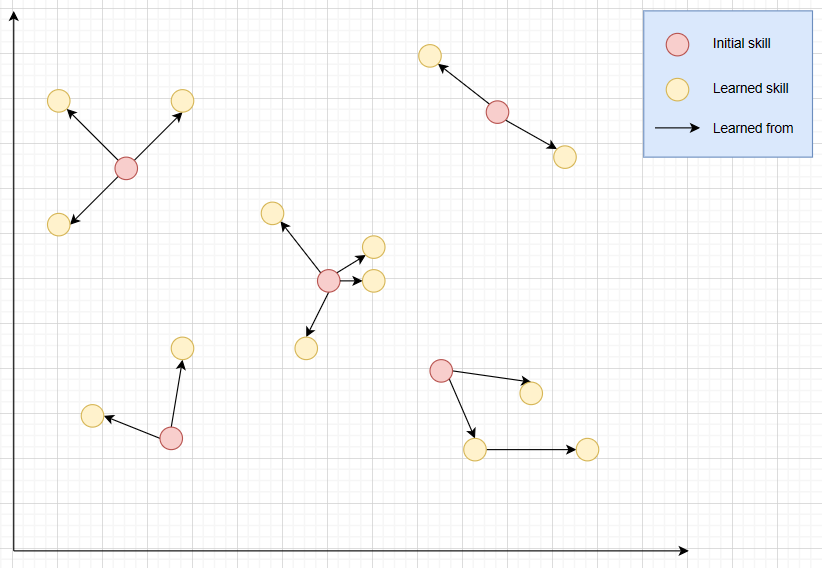
\includegraphics[width=\textwidth]{figures/graph_spread.PNG}
%         \caption{Diverse initial skill set}
%     \end{subfigure}
%     \hfill
%     \begin{subfigure}[b]{0.45\textwidth}
%         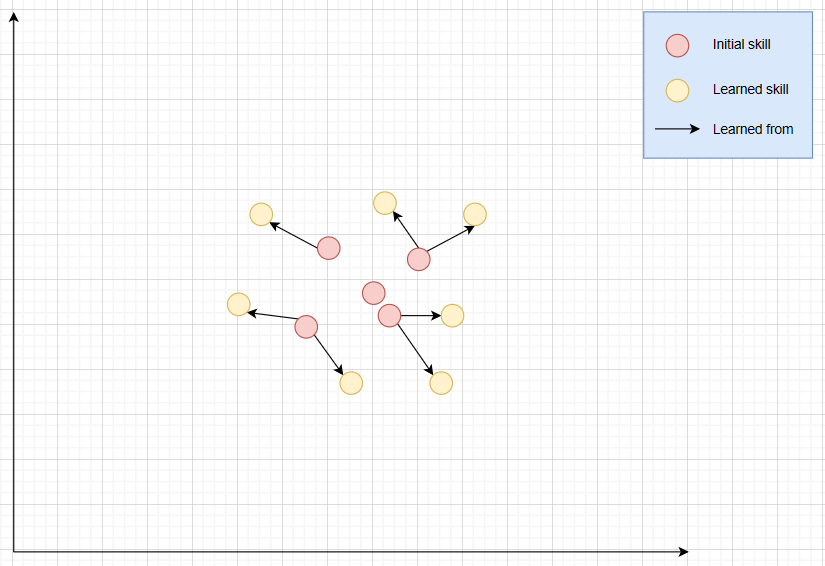
\includegraphics[width=\textwidth]{figures/graph_narrow.PNG}
%         \caption{Narrow initial skill set.}
%     \end{subfigure}
%     \caption{Simplified diagram of trajectory search space.}
%     \label{fig:trajectory-space}
% \end{figure}

% In Figure \ref{fig:trajectory-space} nodes of the graph represent the trajectories which succeed in performing some task and are saved as a skill. Edges represent that the child skill was learned by augmenting the parent skill. Nodes with no parent are the initial skill set, coloured red.